
\part*{Ejercicio 6}
Se nos pidió implementar un Flip-Flop D y un Latch SR a partir de compuertas lógicas discretas, medir sus parámetros que consideramos importantes para la caracterización de su funcionamiento y comparar con equivalentes comerciales. Para verificar las tablas características de funcionamiento de los dispositivos se utilizó una placa experimental Arduino UNO para programar las distintas configuraciones de señales de entrada, y se midieron señales de entrada y salida en un osciloscopio digital. 

\subsection*{Latch SR}
Para la implementación del Latch SR se siguió el diseño del \emph{Gated SR Latch}, encontrado en la sección 5.2 de \emph{Fundamentals of Digital Logic with Verilog Design}, el mismo se muestra en la Figura \ref{6_fig1}. El dispositivo se implemetó utilizando compuertas NAND 74HC00, de tecnología CMOS.



\begin{figure}[H]
\centering
\begin{circuitikz}[scale=1] \draw
(0,0) node[nand port](nandR){}
(0,4) node[nand port](nandS){}
(3,0.28) node[nand port](nandR2){}
++(right:0.7) node(nodo_Q){}
(nandR2.out) to[short, -o] ++(right:2) node[right]{$\bar{Q}$}
(3,3.72) node[nand port](nandS2){}
++(right:0.7) node(nodoQ){}
(nandS2.out) to[short, -o] ++(right:2) node[right]{Q}
(nandR.out) -| (nandR2.in 2)
(nandS.out) -| (nandS2.in 1)
(nandR2.in 1) to[short] ++(-0.5,0) to[short] ++(0,0.7) to[short] ++(2.5,1.5) coordinate(r)
(nandS2.in 2) to[short] ++(-0.5,0) to[short] ++(0,-0.7) to[short] ++(2.5,-1.5) coordinate(s)
(s) to[short,-*] (s|-nodo_Q)
(r) to[short,-*] (s|-nodoQ)

(nandS.in 2) to[short] ++(left:0.5) coordinate (s2)
(nandR.in 1) to[short] ++(left:0.5) coordinate (r2)
(r2) to[short] (r2|-s2)
(-3,2) coordinate (clk)
(clk) node[left](){Clk}
(clk) to[short, o-*] (clk-|s2)
(nandS.in 1) to[short, -o] (nandS.in 1-|clk) node[left](){S}
(nandR.in 2) to[short, -o] (nandR.in 2-|clk) node[left](){R}
;
\end{circuitikz}
\caption{Latch SR implementado} \label{6_fig1}
\end{figure}



Se analizó su correcto funcionamiento para las distintas configuraciones de señales de entrada, y se obtuvo la siguiente tabla característica:

\begin{center}
\begin{tabular}{ccc|c}
Clk & S & R & Q(t+1) \\ 
\hline 
0 & x & x & Q(t) \\ 
1 & 0 & 0 & Q(t) \\ 
1 & 1 & 0 & 1 \\ 
1 & 0 & 1 & 0 \\ 
1 & 1 & 1 & ? \\
\end{tabular} 
\end{center}

\begin{figure}[H]
\begin{center}
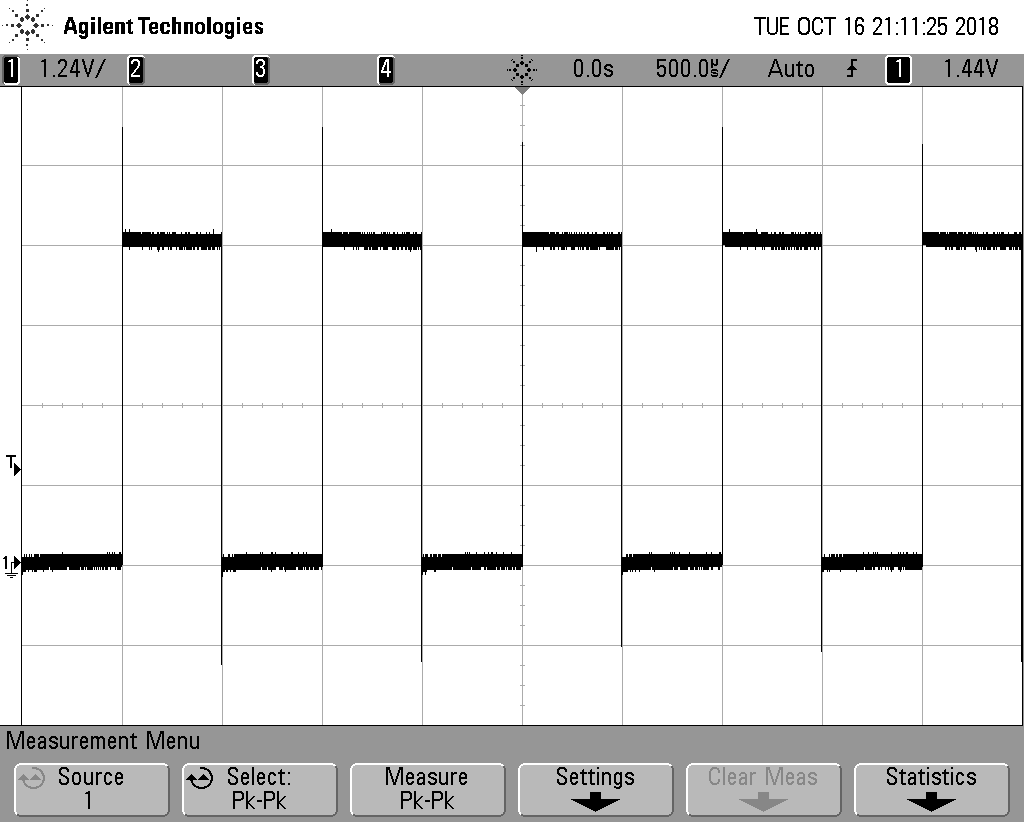
\includegraphics[scale=0.25]{ejercicio6/sr_1.png}
\caption{Estado inestable del Latch SR} \label{6_fig4}
\end{center}
\end{figure}

Las respuestas obtenidas para las distintas configuraciones coinciden con los valores teóricos esperados. Sin embargo, como lo indica el análisis del circuito, la configuración de señales de entrada $Clk=1$, $S=1$ y $R=1$ presenta una inestabilidad, en la cual el valor de salida $Q(t=1)$ no se establece en ningún valor. Para esta configuración, se registró en la Figura \ref{6_fig4} la forma de la salida.

En cuanto a los tiempos de respuesta de la compuerta, se midieron los tiempos de rise, fall y propagación, obteniendose los siguientes valores:

\begin{center}
\begin{tabular}{|c|c|}
\hline 
Rise Time & 27.6 nseg \\ 
\hline 
Fall Time & 26.8 nseg \\ 
\hline 
Propagación & 12.7 nseg \\ 
\hline 
\end{tabular} 
\end{center}

Se buscaron integrados comerciales de tecnología CMOS que implementen un Latch SR para comparar los parámetros medidos. El integrado CD4043 hallado es un integrado 3-state, motivo por el cual, quizás, difieran sus parámetros de los nuestros. Los tiempos de respuesta presentes en la hoja de datos del CD4043 son:

\begin{center}
\begin{tabular}{|c|c|}
\hline 
Rise Time & 100 nseg \\ 
\hline 
Fall Time & 100 nseg \\ 
\hline 
Propagación & 150 nseg \\ 
\hline 
\end{tabular} 
\end{center}


\subsection*{Flip-Flop D}
Para la implementación del Flip-Flop D, se siguió al igual que para el Latch SR el diseño presentado en la sección 5.3 y 5.4 de \emph{Fundamentals of Digital Logic with Verilog Design}. Se utilizó la configuración de dos Latch D master-slave, para lograr un Flip-Flop D activado por flanco ascendente. 

\begin{figure}[H]
\centering
\begin{circuitikz}[scale=1] \draw
(0,0) node[nand port](nandR){}
(0,4) node[nand port](nandS){}
(3,0.28) node[nand port](nandR2){}
++(right:0.7) node(nodo_Q){}
(nandR2.out) to[short, -o] ++(right:2) node[right]{$\bar{Q}$}
(3,3.72) node[nand port](nandS2){}
++(right:0.7) node(nodoQ){}
(nandS2.out) to[short, -o] ++(right:2) node[right]{Q}
(nandR.out) -| (nandR2.in 2)
(nandS.out) -| (nandS2.in 1)
(nandR2.in 1) to[short] ++(-0.5,0) to[short] ++(0,0.7) to[short] ++(2.5,1.5) coordinate(r)
(nandS2.in 2) to[short] ++(-0.5,0) to[short] ++(0,-0.7) to[short] ++(2.5,-1.5) coordinate(s)
(s) to[short,-*] (s|-nodo_Q)
(r) to[short,-*] (s|-nodoQ)

(nandS.in 2) to[short] ++(left:0.5) coordinate (s2)
(nandR.in 1) to[short] ++(left:0.5) coordinate (r2)


(r2) to[short] (r2|-s2)
(-5,2) coordinate(clk)
(clk) node[left](){Clk}
(clk) to[short, o-*] (clk-|s2)
(nandS.in 1) to[short, -o] (nandS.in 1-|clk) node[left](nodoS){D}
(-3,-0.28) node[american not port](notS){}
(notS.out) to[short] (nandR.in 2)
(notS.in) to[short] ++(left:0.5) coordinate(notin)
(notin) to[short,-*] (notin|-nodoS)

;
\end{circuitikz}
\caption{Modulo Latch D} \label{6_fig2}
\end{figure}

En la Figura \ref{6_fig2} se muestra la implementación de un módulo Latch D, el cual se utilzará, como se explicó para implementar el Flip-Flop D, ilustrado en la Figura \ref{6_fig3}


\begin{figure}[H]
\centering
\begin{circuitikz}[scale=1] \draw
(0,0) node[draw,minimum width=2cm,minimum height=2.4cm,anchor=south west]{}
(5,0) node[draw,minimum width=2cm,minimum height=2.4cm,anchor=south west]{}

(0,0.6) node[right](Clkm){Clk}
(0,1.8) node[right](Dm){D}
(2,0.6) node[left](Qm_){$\bar{Q}$}
(2,1.8) node[left](Qm){Q}



(5,0.6) node[right](Clks){Clk}
(5,1.8) node[right](Ds){D}
(7,0.6) node[left](Qs_){$\bar{Q}$}
(7,1.8) node[left](Qs){Q}

;
\draw
[thick,dashed] (-2,-2.5) rectangle (8,3);

\draw
(0,1.8) to[short,-o] ++ (left:3) node[left](D){D}
(0,0.6) to[short,-o] ++ (left:3) node[left](clk){Clk}

(-1,0.6) to[short,*-] ++(down:2) to [short] ++(right:1) node(notin){}
++(right:1)node[american not port](not){}
(notin) to[short] (not.in)
(not.out) to[short] ++(right:2) node(notout){}
(notout) to[short,-] (notout|-Clks)
to[short] (5,0.6)

(2,1.8) to[short] (5,1.8)

(7,1.8) to[short,-o] ++(right:2) node[right](Q){Q}
(7,0.6) to[short,-o] ++(right:2) node[right](noQ){$\bar{Q}$}
;
\end{circuitikz}
\caption{Diagrama Flip-Flop D} \label{6_fig3}
\end{figure}

La respuesta de las salidas en función a las entradas fue la esperada, cumpliéndose la siguiente tabla característica de un Flip-Flop D de flanco ascendente:

\begin{center}
\begin{tabular}{cc|c}
Clk & D & Q(t+1) \\ 
\hline 
\texttiming[timing/c/rising arrows, timing/c/arrow pos=.7]{2{C}} & 0 & 0 \\ 
\texttiming[timing/c/rising arrows, timing/c/arrow pos=.7]{2{C}} & 1 & 1 \\ 
\texttiming[timing/c/falling arrows, timing/c/arrow pos=.7]{HC}  & x & Q(t) \\
\end{tabular} 
\end{center}

Se midieron los tiempos de rise, fall y de propagación. Se obtuvieron los siguientes resultados:


\begin{center}
\begin{tabular}{|c|c|}
\hline 
Tiempo de Propagación & 18.8 nseg \\ 
\hline 
Rise Time & 27.8 nseg \\ 
\hline 
Fall Time & 27.6 nseg \\ 
\hline 
\end{tabular} 
\end{center}

Los resultados obtenidos se contrastan con los datos provistos por la hoja de datos del integrado comercial 74HC74, que implementa un Flip-Flop D. Los tiempos de propagación y de transición que se especifican son:

\begin{center}
\begin{tabular}{|c|c|}
\hline 
Tiempo de Propagación & 17 nseg \\ 
\hline 
Tiempo de Transición & 7 nseg \\ 
\hline 
\end{tabular} 
\end{center}

La diferencia apreciada entre los tiempos de transición medidos y los especificados en la hoja de datos del integrado comercial, puede deberse a que los tiempos de transición de las señales provistas por el Arduino UNO son significativamente mayores a los tiempos de respuesta de las compuertas utilizadas para implementar el Flip Flop, por lo tanto esto induce un error en la medición. 
